% TU Delft beamer template
% Author: Erwin Walraven (initial version was created by Maarten Abbink)
% Delft Universiy of Technology

\documentclass{beamer}
%\usepackage[english]{babel}
%\usepackage{calc}
%\usepackage[absolute,overlay]{textpos}
%\usepackage{graphicx}
%\usepackage{subfig}
%\usepackage{amsmath}
%\usepackage{amsfonts}
%\usepackage{amsthm}
%\usepackage{mathtools}
%\usepackage{comment}
%\usepackage{MnSymbol,wasysym}


%\setbeamertemplate{navigation symbols}{} % remove navigation symbols
%\mode<presentation>{\usetheme{tud}}
\usetheme{Madrid}
\usecolortheme{beaver}


\usepackage{multirow}
\usepackage{makecell}
\renewcommand{\footnotesize}{\fontsize{7pt}{9pt}\selectfont}

\usepackage{tikzsymbols}

\setbeamertemplate{caption}[numbered]

\usepackage{subfig}

\makeatletter       % for rom in deal.ii symbol
\newcommand*{\rom}[1]{\expandafter\@slowromancap\romannumeral #1@}
\makeatother

\usepackage[utf8]{inputenc}
\usepackage{lmodern}


\title[]{Report on the 2D Paper}
\institute[]{Delft University of Technology, the Netherlands}
\author{Jie Liu}
%\date{}

\begin{document}
{
\setbeamertemplate{footline}{\usebeamertemplate*{minimal footline}}
\frame{\titlepage}
}

\section{Introduction}
\begin{frame}
\frametitle{Problem statement}
\vspace{-7em}
\begin{block}{Equation to be solved}
\scriptsize
\begin{equation}
 \nabla \cdot (T_1 \nabla u) + T_2 \frac{\partial{u}}{\partial{x}} + T_3 \frac{\partial{u}}{\partial{y}} + T_4 u = f,\qquad (x,y) \in \Omega = [0,\,1] \times [0,\,1],
 \label{problem_to_be_investigated}
\end{equation}
where $T_1$, $T_2$, $T_3$ and $T_4$ are coefficient functions\footnote{$T_2$ and $T_3$ have not been included practically in the code yet.}. The solution $u$ can be both real-valued and complex-valued if not stated otherwise. By choosing different $T_i$, we can have Poisson, diffusion or Helmholtz problems.
\end{block}
\end{frame}

\begin{frame}{Aim of the second paper}
\vspace{-6em}
\begin{enumerate}
 \item To determine $\alpha_{\rm R}$ and $\beta_{\rm R}$ for different FEM methods of different FEM packages for various 2D problems.
 \item To choose FEM methods/elements that give smaller round-off error, i.e. $\alpha_{\rm R}$ and $\beta_{\rm R}$.
 \item To apply the strategy in the 1D paper to find the optimal number of DoFs of 2D problems$^{*}$.
\end{enumerate}
Note that, we may not need to improve the legacy code of the mature software.
\end{frame}



\begin{frame}{FEM Status}
\vspace{-3em}
The status of the application of FEM methods of different FEM packages, including deal.\rom{2} and FEniCS, on various Eq.~(\ref{problem_to_be_investigated}) is shown in Table~\ref{table_status_fem_application}.
\begin{table}[!ht]
\scriptsize
\begin{tabular}{ l | c | c}
 & deal.\rom{2} & FEniCS \\ \hline
 Standard FEM ($P_p$) & $\Smiley$\footnote{Working well.} & -- \\ \hline
 Mixed FEM ($RT_p/P_{p}^{\rm disc}$) & $\Smiley$ & -- \\ \hline
 Mixed FEM ($BDM_p/Q_{p-1}^{\rm disc}$)\footnote{The notation $Q$ is based on the notation in the deal.\rom{2} code.} & $\Smiley$ & $\Smiley$\footnote{Only applied on Eq.~(\ref{sample_equation}), see the next slide.}
\end{tabular}
\caption{Status of application of FEM methods. The element degree $p$ can be of different order if not stated otherwise.}
\label{table_status_fem_application}
\end{table}
\end{frame}

\begin{frame}{A particular case for FEniCS}
\vspace{-3em}
We consider the following case for implementing $BDM$ elements in FEniCS.
\begin{block}{A case for FEniCS}
\begin{equation}
 -\Delta u = -4,
 \label{sample_equation}
\end{equation}
with the solution $u=1+(x-0.5)^2+(y-0.5)^2$.
The left and right boundaries of the unit square is imposed by Dirichlet boundary conditions, while the upper and bottom boundaries are imposed by Neumman boundary conditions, i.e. $\mathbf{v}=(-2\cdot(x-0.5)), -2\cdot(y-0.5))$.
\end{block}
An illustration of the solution for $BDM_2/Q_1^{\rm disc}$ elements is shown in Fig.~\ref{results_fenics} in the next slide.
\end{frame}

\begin{frame}{Results obtained from FEniCS}
\vspace{-3em}
\begin{figure}
\subfloat[][Magnitude of $\mathbf{v}~(2\sqrt{(x-0.5)^2+(y-0.5)^2})$]{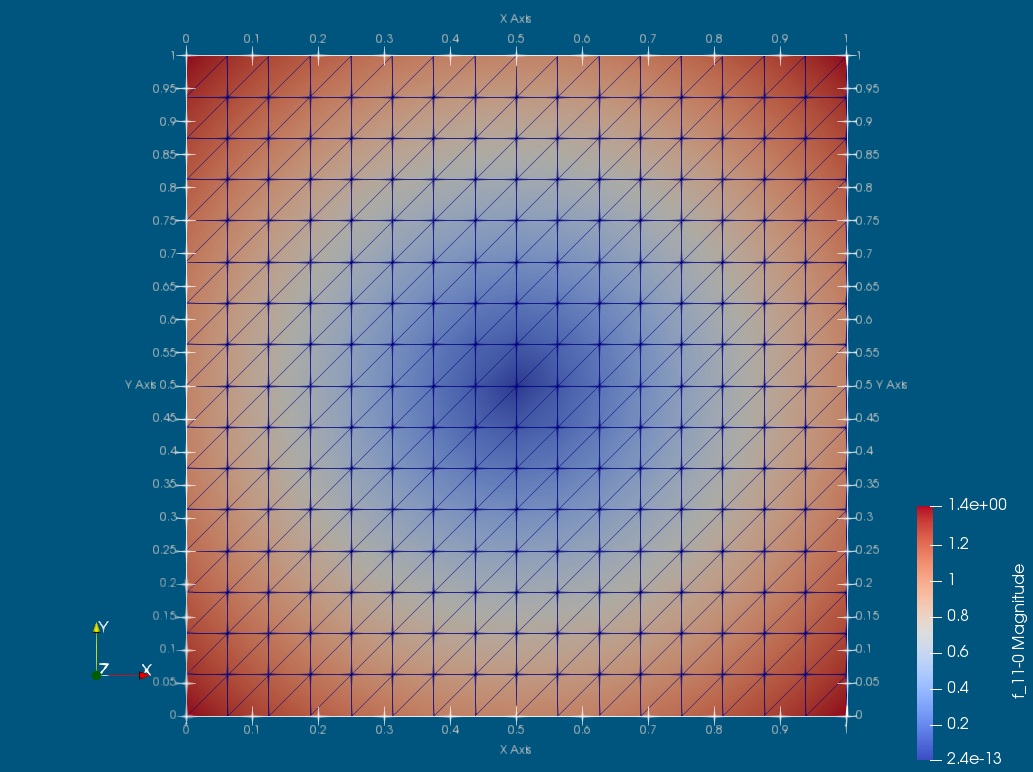
\includegraphics[width=0.5\linewidth]{image/mixed-poisson_sigma_custom.png}}
\subfloat[][$\mathbf{u}~(1+(x-0.5)^2+(y-0.5)^2)$]{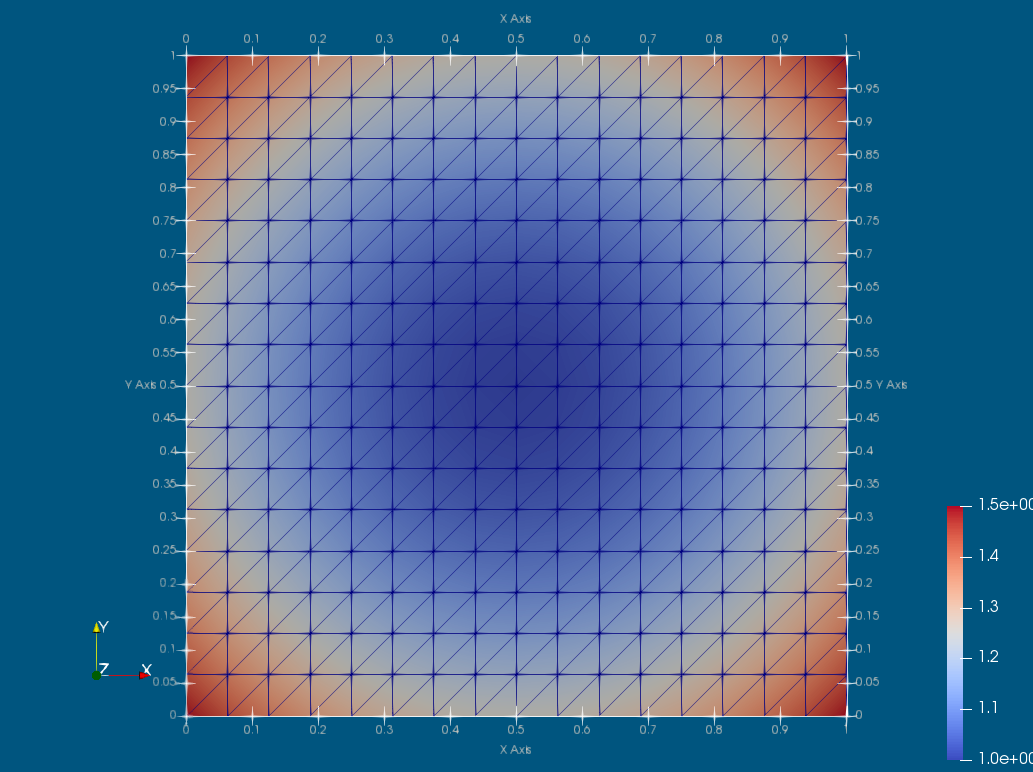
\includegraphics[width=0.5\linewidth]{image/mixed-poisson_u_custom.png}}
\caption{Solution of Eq.~(\ref{sample_equation}) obtained from applying $BDM_2/Q_1^{\rm disc}$ elements in FEniCS.}
\label{results_fenics}
\end{figure}
\end{frame}


\section{Progress}
\begin{frame}{Progress}
\vspace{-3.5em}
\begin{block}{deal.\rom{2}}
\begin{itemize}
 \item The latest version of deal.\rom{2} (9.2.0) works. However, the problem of higher-order $BDM$ elements still exists, i.e. $p\leq 7$\footnote{The specific function that gives an error is PolynomialsP$\langle2\rangle$::create\_polynomial\_ordering()}.
 \item There is also a limitation for the degree of $RT$ elements in deal.\rom{2}, which is $p\leq 13$.
 \item For $P$ elements, $p$ can be as large as 515.
\end{itemize}
\end{block}
\begin{block}{FEniCS}
\begin{itemize}
 \item The round-off error of the standard FEM is analyzed with the order of convergence being correct.
\end{itemize}
\end{block}
\end{frame}


\section{Discussion}
\begin{frame}{Discussion}
\vspace{-9em}
\begin{enumerate}
 \item Results of FEniCS or IGA as a supplement?
 \item Using the relative error instead of the absolute error for the 2D case? 
 \item Super convergence common when using 2D mixed FEM methods solving a 1D problem?
\end{enumerate}
\end{frame}


\section{Future work}
\begin{frame}{Future work}
\vspace{-10em}
\begin{itemize}
 \item To consider $T_2$ and $T_3$, i.e. first-order parts, of Eq.~(\ref{problem_to_be_investigated}) in deal.\rom{2}.
 \item To integrate the function for computing the errors in FEniCS.
 \item To verify the accuracy of $BDM_p/DGQ_{p-1}^{\rm disc}$ elements for $p=7$ because the round-off of different equations is not regular.
\end{itemize}
\end{frame}

\section{Next topic}
\begin{frame}{Topics of the third paper}
\vspace{-11em}
\begin{enumerate}
 \item Resolving boundary layers and/or construct a method to avoid these boundary layers~\cite{kumar2016three}.
 \item 2D lagrangian polynomials not the same order in each direction?
\end{enumerate}
\end{frame}

\bibliographystyle{unsrt}
\bibliography{bibfile_presentation}

\end{document}
